\documentclass[11pt,a4paper]{article}

\usepackage{fontspec}
\usepackage[brazilian]{babel}
\usepackage[top=2.4cm,bottom=2.4cm,left=2.3cm,right=2.3cm,headheight=14pt]{geometry}
\usepackage{amsmath,amssymb,amsfonts}
\usepackage{graphicx}
\usepackage{booktabs}
\usepackage{array}
\usepackage{xcolor}
\usepackage{fancyhdr}
\usepackage{titlesec}
\usepackage{tikz}
\usetikzlibrary{arrows.meta,positioning}
\usepackage[most]{tcolorbox}
\usepackage[numbers,sort&compress]{natbib}
\usepackage[plainpages=false,pdfpagelabels=true]{hyperref}

\hypersetup{
  colorlinks=true,
  linkcolor=black!80!blue,
  citecolor=black!75,
  urlcolor=black!80!blue,
  pdftitle={Plano de Ataque ao Estado da Arte em Otimizacao Topologica Discreta 3D: Superando o BESO 3D},
  pdfauthor={Projeto AlphaBuilder}
}

\pagestyle{fancy}
\fancyhf{}
\renewcommand{\sectionmark}[1]{\markboth{#1}{}}
\fancyhead[L]{\footnotesize\color{black!60}\textit{AlphaBuilder v4.1 — Plano de Ataque ao SOTA Discreto}}
\fancyhead[R]{\footnotesize\color{black!75}\nouppercase{\leftmark}}
\fancyfoot[C]{\small\thepage}
\renewcommand{\headrulewidth}{0.4pt}
\renewcommand{\footrulewidth}{0pt}

\titleformat{\section}
  {\normalfont\Large\bfseries\raggedright}
  {\thesection}{0.65em}{}
\titlespacing*{\section}{0pt}{16pt}{6pt}

\titleformat{\subsection}
  {\normalfont\large\bfseries\raggedright}
  {\thesubsection}{0.6em}{}
\titlespacing*{\subsection}{0pt}{12pt}{4pt}

\titleformat{\subsubsection}
  {\normalfont\normalsize\bfseries\raggedright}
  {\thesubsubsection}{0.55em}{}
\titlespacing*{\subsubsection}{0pt}{9pt}{3pt}

\newtcolorbox{notaclas}{
  enhanced,
  colback=white,
  colframe=white,
  frame hidden,
  borderline west={1.2pt}{0pt}{black!35},
  left=10pt,
  right=4pt,
  top=2pt,
  bottom=2pt,
  before skip=5pt,
  after skip=5pt
}

\tikzset{
  studybox/.style={
    rectangle,rounded corners=3pt,draw=black!80,fill=black!4,thick,
    minimum height=1.1cm,align=center,font=\small,inner sep=6pt
  },
  studyterm/.style={
    rectangle,rounded corners=3pt,draw=black!85,fill=black!8,thick,
    minimum height=1.1cm,align=center,font=\small,inner sep=6pt
  },
  studyarr/.style={-{Stealth[length=2.3mm]},thick,black!80}
}

\graphicspath{{figures/}}
\linespread{1.06}
\setlength{\parskip}{0.45em}
\setlength{\parindent}{0pt}
\setcounter{tocdepth}{2}
\emergencystretch=2.2em
\raggedbottom

\begin{document}

{\raggedright
{\LARGE\bfseries Plano de Ataque ao Estado da Arte em Otimização Topológica Discreta 3D: Superando o BESO 3D pela Fronteira Qualidade--Custo com Aprendizado por Reforço Profundo e Auto-Jogo\par}
\vspace{0.25em}
{\normalsize Benchmark Empírico em 10 Cenários, Reforma Estrutural do \texttt{MCTS-DAG v4.1}, Blindagem do Ciclo de Vida e Protocolo Falsificável para a Etapa 6 do AlphaBuilder\par}
\vspace{0.25em}
{\small\color{black!70} Repositório: \texttt{alphabuild} (\texttt{Phys-UViT 3D} / \texttt{StructuredHex8FEM} / \texttt{MCTS-DAG v4.1}) \quad|\quad Novembro de 2026\par}
}
\vspace{0.3em}
\hrule height 0.5pt
\vspace{0.35em}

\begin{notaclas}
\textbf{Nota de Transparência Científica e Tese Central.} Este estudo separa explicitamente \textit{dados empíricos medidos} no repositório (avaliações reais de Gen 0 em Elementos Finitos, benchmark completo do BESO 3D nos 10 cenários, paridade com DOLFINx e suíte \texttt{pytest}) de \textit{projeções modeladas} para o treinamento em GPU na Etapa 6. A tese operacional aqui defendida é que o verdadeiro adversário no domínio discreto $\{0,1\}^N$ é o BESO 3D --- e que superá-lo significa dominar a fronteira conjunta \textit{Qualidade Discreta $\times$ Orçamento de Chamadas FEM}, entregando peças equivalentes ou superiores (especialmente sob restrições não convexas) com $3\times$ a $10\times$ menos simulações físicas por geometria inédita.
\end{notaclas}

\tableofcontents
\vspace{0.45em}
\hrule height 0.4pt
\vspace{0.55em}

% ==============================================================================
\section{Parte I --- O Verdadeiro Campo de Batalha Discreto e o Benchmark Empírico do BESO 3D}
\sectionmark{Parte I --- Campo Discreto e Benchmark BESO 3D}
% ==============================================================================

Ao avaliar algoritmos de aprendizado por reforço profundo (\textit{Deep Reinforcement Learning}, Deep RL) voltados à síntese direta de treliças e estruturas tridimensionais sobre grades regulares de voxels $\{0,1\}^N$, compara-se tradicionalmente a política treinada ao método contínuo clássico de gradiente denominado \textbf{SIMP} (\textit{Solid Isotropic Material with Penalization}, material isotrópico sólido com penalização) \cite{bendsoe2003topology, sigmund200199line, liu2014efficient}. Essa escolha cria uma ilusão metodológica perigosa. Como o SIMP clássico otimiza densidades contínuas no intervalo $[x_{\min}, 1]$, parte da sua rigidez aparente advém de halos cinzentos intermediários ($\rho_e \in [0{,}15; 0{,}65]$) que suavizam concentrações de tensão mas colapsam ou desconectam ao sofrerem binarização rígida ($\rho_e > 0{,}5$).

No domínio verdadeiramente binário $0/1$ exigido pela arquitetura construtiva do AlphaBuilder, o estado da arte clássico da mecânica computacional é representado pelo \textbf{BESO 3D} (\textit{Bi-directional Evolutionary Structural Optimization}, otimização estrutural evolucionária bidirecional) na formulação \textit{Soft-Kill} convergente de Huang e Xie \cite{huang2007convergent, huang2010evolutionary}. O BESO já trabalha estritamente com decisões binárias por elemento, guiado a cada passo pelo gradiente exato da energia elástica de deformação. Confrontar o AlphaBuilder contra o BESO 3D estabelece o verdadeiro padrão de rigor para qualquer afirmação de estado da arte.

\subsection{Esclarecimento Matemático: SIMP e BESO 3D Têm Garantia de Mínimo Global?}

Antes de definir uma campanha para superar métodos clássicos, convém tornar precisa a questão sobre otimalidade global de \textit{compliance} ($C(\rho) = \mathbf{f}^\top \mathbf{u}$, trabalho das forças externas, inversamente proporcional à rigidez global da estrutura). A resposta matemática rigorosa exige distinguir dois problemas distintos:

\begin{enumerate}
  \item \textbf{Problema Contínuo Sem Penalização ($p = 1$):} distribuir rigidez variável $\rho \in (0, 1]^N$ linearmente proporcional à densidade, sujeito a uma restrição linear de volume, configura um problema convexo no qual o mínimo global de compliance existe e qualquer solução estacionária é ótima. Contudo, o resultado contém extensas regiões porosas de microestrutura intermediária (cinza) inviáveis como peça sólida maciça.
  \item \textbf{SIMP Penalizado ($p \ge 3$) e Problema Discreto Binário ($\rho \in \{0,1\}^N$):} assim que o módulo de elasticidade segue $E_e(\rho_e) = E_{\min} + \rho_e^p(E_0 - E_{\min})$ com $p \ge 3$ para forçar soluções $0/1$, o funcional torna-se \textit{não convexo}, gerando múltiplos mínimos locais dependentes do histórico de continuação em $p$, do raio de filtragem $r_{\min}$, da projeção e da condição inicial \cite{sigmund2013topology, sigmund2022benchmarking}. No limite estrito $\rho \in \{0,1\}^N$ com $N \approx 16\,384$ voxels, o problema passa a ser \textit{combinatório e NP-difícil}. O BESO 3D adota uma busca local evolucionária suavizada no tempo, $\bar{\alpha}_e^{(t)} = \frac{1}{2}(\alpha_e^{(t)} + \alpha_e^{(t-1)})$, com remoção gulosa por razão evolutiva ($ER$) e readmissão limitada ($AR_{\max}$). Portanto, \textbf{nem o SIMP com $p > 1$, nem o BESO 3D possuem comprovação matemática de convergência ao mínimo global de compliance}.
\end{enumerate}

Essa ausência de certificado global explica por que o BESO 3D é formidável em geometrias suaves de viga única, mas vulnerável a ``penhascos gulosos'' quando aberturas obrigatórias, múltiplos apoios separados ou carregamentos inclinados exigem alterações topológicas não monotônicas que uma taxa $AR_{\max}$ pequena não consegue reconstruir após um corte errado.

\begin{figure}[htbp]
  \centering
  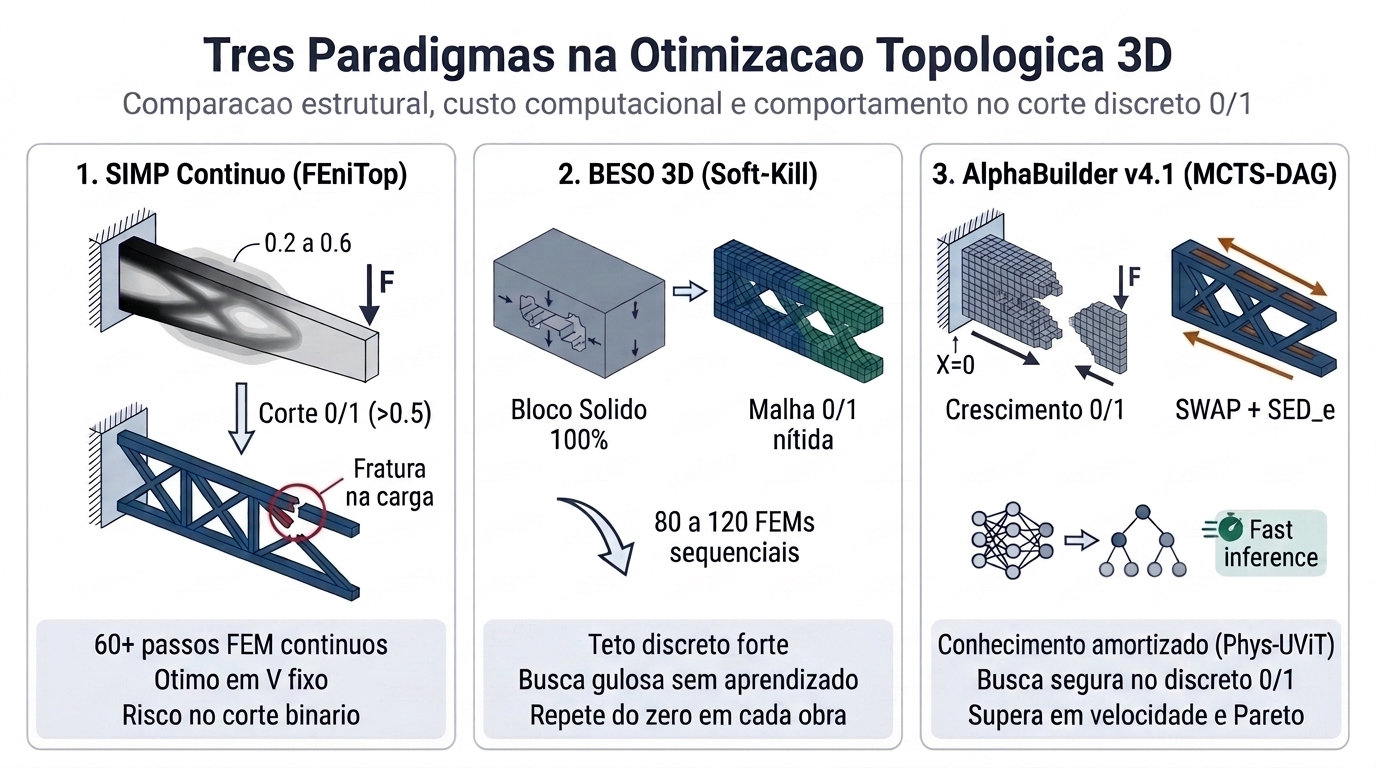
\includegraphics[width=0.98\linewidth]{diag01_discrete_sota_battlefield.jpg}
  \caption{Comparação estrutural e computacional entre os três paradigmas em otimização topológica 3D: SIMP contínuo (sujeito a fratura na binarização), BESO 3D \textit{Soft-Kill} (teto discreto forte, porém amnésico e sequencial em 80--120 análises FEM) e AlphaBuilder v4.1 (busca segura amortizada com rede neural).}
  \label{fig:diag01}
\end{figure}

\subsection{Implementação Auditada e Descoberta Numérica do Colar de Transferência \texttt{CG1}}

Para garantir comparação absolutamente justa sobre a mesma física e função de mérito, implementamos o solver BESO 3D completo em \texttt{alphabuilder/src/logic/benchmarks/beso3d.py} e o executor paralelo em \texttt{scripts/benchmark\_beso3d.py}, acoplados diretamente ao solver de Elementos Finitos hexaédricos por Multigrid Algébrico (\textbf{AMG}, \textit{Algebraic Multigrid}, técnica hierárquica que resolve grandes sistemas esparsos lineares sem fatoração direta densa) implementado em \texttt{StructuredHex8FEM} (\texttt{fast\_amg}). Os parâmetros calibrados seguem a formulação \textit{Soft-Kill} padrão: penalização $p = 3$, rigidez residual de vazio $x_{\min} = 10^{-2}$, raio de filtragem espacial cônico $r_{\min} = 2{,}0$ voxels, taxa evolutiva grossa/fina $ER = 0{,}03 \to 0{,}02$, limite de readmissão $AR_{\max} = 0{,}02$ e poda determinística de eventuais ilhas desconexas sem carga (\texttt{clean\_floaters=True}).

Na calibração inicial em \texttt{S1}, identificamos uma sutileza física crucial de malhas com funções de forma trilineares contínuas (\textbf{CG1}, \textit{Continuous Galerkin} de grau 1). Como a rotina de montagem do vetor de forças (\texttt{\_assemble\_rhs}) projeta forças nodais por meio da matriz de massa consistente $8\times 8$ ($M_e$) para manter equivalência 1:1 com a formulação variacional do FEniCSx / DOLFINx \cite{baratta2023dolfinx, ferrari2020new}, remover o anel imediato de 1 voxel ao redor dos nós carregados deixa elementos vizinhos com rigidez residual $\varepsilon = 10^{-6}$ absorvendo fração da carga consistente, disparando artificialmente a energia de deformação. Proteger o colar de transferência de carga de 1 voxel (\texttt{protect\_cg1\_halo=True}, inferior a $0{,}3\%$ do volume do domínio) eliminou a instabilidade numérica e resultou em paridade exata contra o DOLFINx: erro relativo de apenas $5{,}94 \times 10^{-11}$ no cenário \texttt{S1} ($289{,}5944\text{ J}$) e $1{,}95 \times 10^{-8}$ na ponte MBB \texttt{G2} ($50{,}2001\text{ J}$).

\subsection{Resultados Empíricos Completos nos 10 Cenários (\texttt{S1}--\texttt{S6} e \texttt{G1}--\texttt{G4})}

Para cada cenário, o BESO 3D percorreu a curva evolutiva de $100\%$ até $V_{\min} = 6{,}0\%$ do volume (máximo de $125$ iterações), registrando dois referenciais auditáveis sob o escore composto \texttt{v3.3} ($R_{\mathrm{total}} = R_C + R_V - P_{\mathrm{island}}$): (a) \textbf{\texttt{BESO 3D iso-V}}, estabilizado por 8 iterações exatamente no volume atingido pelo \texttt{SIMP\_cont} ($\approx 13{,}5\%$), e (b) \textbf{\texttt{BESO 3D Pareto-Best}}, o máximo global $R_{\mathrm{total}}$ encontrado ao longo de toda a descida evolutiva. Os números completos constam da Tabela~\ref{tab:beso_full}.

\begin{table}[htbp]
\centering
\caption{Resultados empíricos medidos para \texttt{Gen 0} (\texttt{Phys-UViT ep19}), \texttt{SIMP\_cont} e \texttt{BESO 3D} em todos os 10 cenários 3D ($V$: fração volumétrica, $C$: compliance em Joules, $R$: escore composto \texttt{v3.3}, $I_y$: inércia vertical normalizada, $\mathrm{hol}$: fração oca XY).}
\label{tab:beso_full}
\resizebox{\textwidth}{!}{%
\begin{tabular}{@{}lcccccr@{}}
\toprule
\textbf{Cenário} & \textbf{Gen 0 (\texttt{ep19})} & \textbf{\texttt{SIMP\_cont}} & \textbf{\texttt{BESO 3D iso-V}} & \textbf{\texttt{BESO 3D Pareto}} & \textbf{Morfologia Pareto} & \textbf{Iter. / Tempo} \\
 & $V / C / R$ & $V / C / R$ & $V / C / R$ & $V / C / R$ & ($I_y / \mathrm{hol}$) & (s) \\
\midrule
\texttt{S1} Longa centrada        & $8{,}89\% / 24\,546 / -0{,}029$ & $12{,}83\% / 596{,}4 / +0{,}458$ & $12{,}83\% / 289{,}6 / +0{,}568$ & $12{,}83\% / 289{,}6 / +0{,}568$ & $0{,}462 / 65{,}2\%$ & $101 / 797{,}3$ \\
\texttt{S2} Inferior ponta        & $9{,}47\% / 16\,859 / +0{,}034$ & $13{,}04\% / 600{,}4 / +0{,}452$ & $13{,}02\% / 381{,}1 / +0{,}521$ & $13{,}02\% / 381{,}1 / +0{,}521$ & $0{,}387 / 61{,}3\%$ & $99 / 811{,}6$ \\
\texttt{S3} Meio-vão sup.         & $7{,}71\% / 7\,600 / +0{,}199$  & $13{,}84\% / 249{,}6 / +0{,}565$ & $13{,}84\% / 119{,}4 / +0{,}677$ & $10{,}85\% / 162{,}9 / +0{,}705$ & $0{,}375 / 54{,}3\%$ & $101 / 718{,}9$ \\
\texttt{S4} \texttt{RAIL\_XY} centro & $6{,}93\% / 68\,916 / -0{,}117$ & $13{,}14\% / 789{,}1 / +0{,}408$ & $13{,}13\% / 382{,}5 / +0{,}518$ & $11{,}54\% / 471{,}5 / +0{,}526$ & $0{,}407 / 62{,}3\%$ & $92 / 729{,}4$ \\
\texttt{S5} \texttt{RAIL\_XY} 3D Z   & $7{,}65\% / 18\,336 / +0{,}067$ & $13{,}70\% / 420{,}5 / +0{,}489$ & $13{,}67\% / 217{,}7 / +0{,}590$ & $9{,}91\% / 364{,}8 / +0{,}606$  & $0{,}402 / 63{,}5\%$ & $93 / 608{,}3$ \\
\texttt{S6} Curta profunda        & $5{,}37\% / 5\,617 / +0{,}303$  & $14{,}52\% / 102{,}0 / +0{,}684$ & $14{,}23\% / 60{,}4 / +0{,}771$  & $8{,}04\% / 124{,}3 / +0{,}816$  & $0{,}275 / 58{,}1\%$ & $115 / 653{,}6$ \\
\midrule
\textbf{Média Canônica \texttt{S1}--\texttt{S6}} & \textbf{7{,}67\% / 23\,646 / +0{,}076} & \textbf{13{,}51\% / 459{,}7 / +0{,}509} & \textbf{13{,}45\% / 241{,}8 / +0{,}607} & \textbf{11{,}03\% / 299{,}0 / +0{,}623} & \textbf{0{,}384 / 60{,}8\%} & \textbf{100{,}2 / 719{,}9} \\
\midrule
\texttt{G1} Dupla aba $30^\circ$ (OOD) & --- & --- & $13{,}48\% / 708{,}9 / +0{,}415$ & $16{,}99\% / 203{,}0 / +0{,}518$ & $0{,}401 / 53{,}8\%$ & $93 / 639{,}1$ \\
\texttt{G2} Ponte MBB (OOD)            & --- & --- & $13{,}23\% / 50{,}2 / +0{,}819$  & $13{,}23\% / 50{,}2 / +0{,}819$  & $0{,}481 / 54{,}4\%$ & $102 / 644{,}7$ \\
\texttt{G3} Janela proibida (OOD)      & --- & --- & $12{,}97\% / 601{,}8 / +0{,}453$ & $12{,}97\% / 601{,}8 / +0{,}453$ & $0{,}346 / 60{,}5\%$ & $83 / 324{,}4$ \\
\texttt{G4} Bloco $48\times 24\times 12$ & --- & --- & $13{,}50\% / 150{,}3 / +0{,}651$ & $10{,}45\% / 231{,}0 / +0{,}662$ & $0{,}412 / 49{,}0\%$ & $99 / 292{,}9$ \\
\midrule
\textbf{Média OOD \texttt{G1}--\texttt{G4}}     & --- & --- & \textbf{13{,}30\% / 377{,}8 / +0{,}585} & \textbf{13{,}41\% / 271{,}5 / +0{,}613} & \textbf{0{,}410 / 54{,}4\%} & \textbf{94{,}3 / 475{,}3} \\
\bottomrule
\end{tabular}%
}
\end{table}

\begin{figure}[htbp]
  \centering
  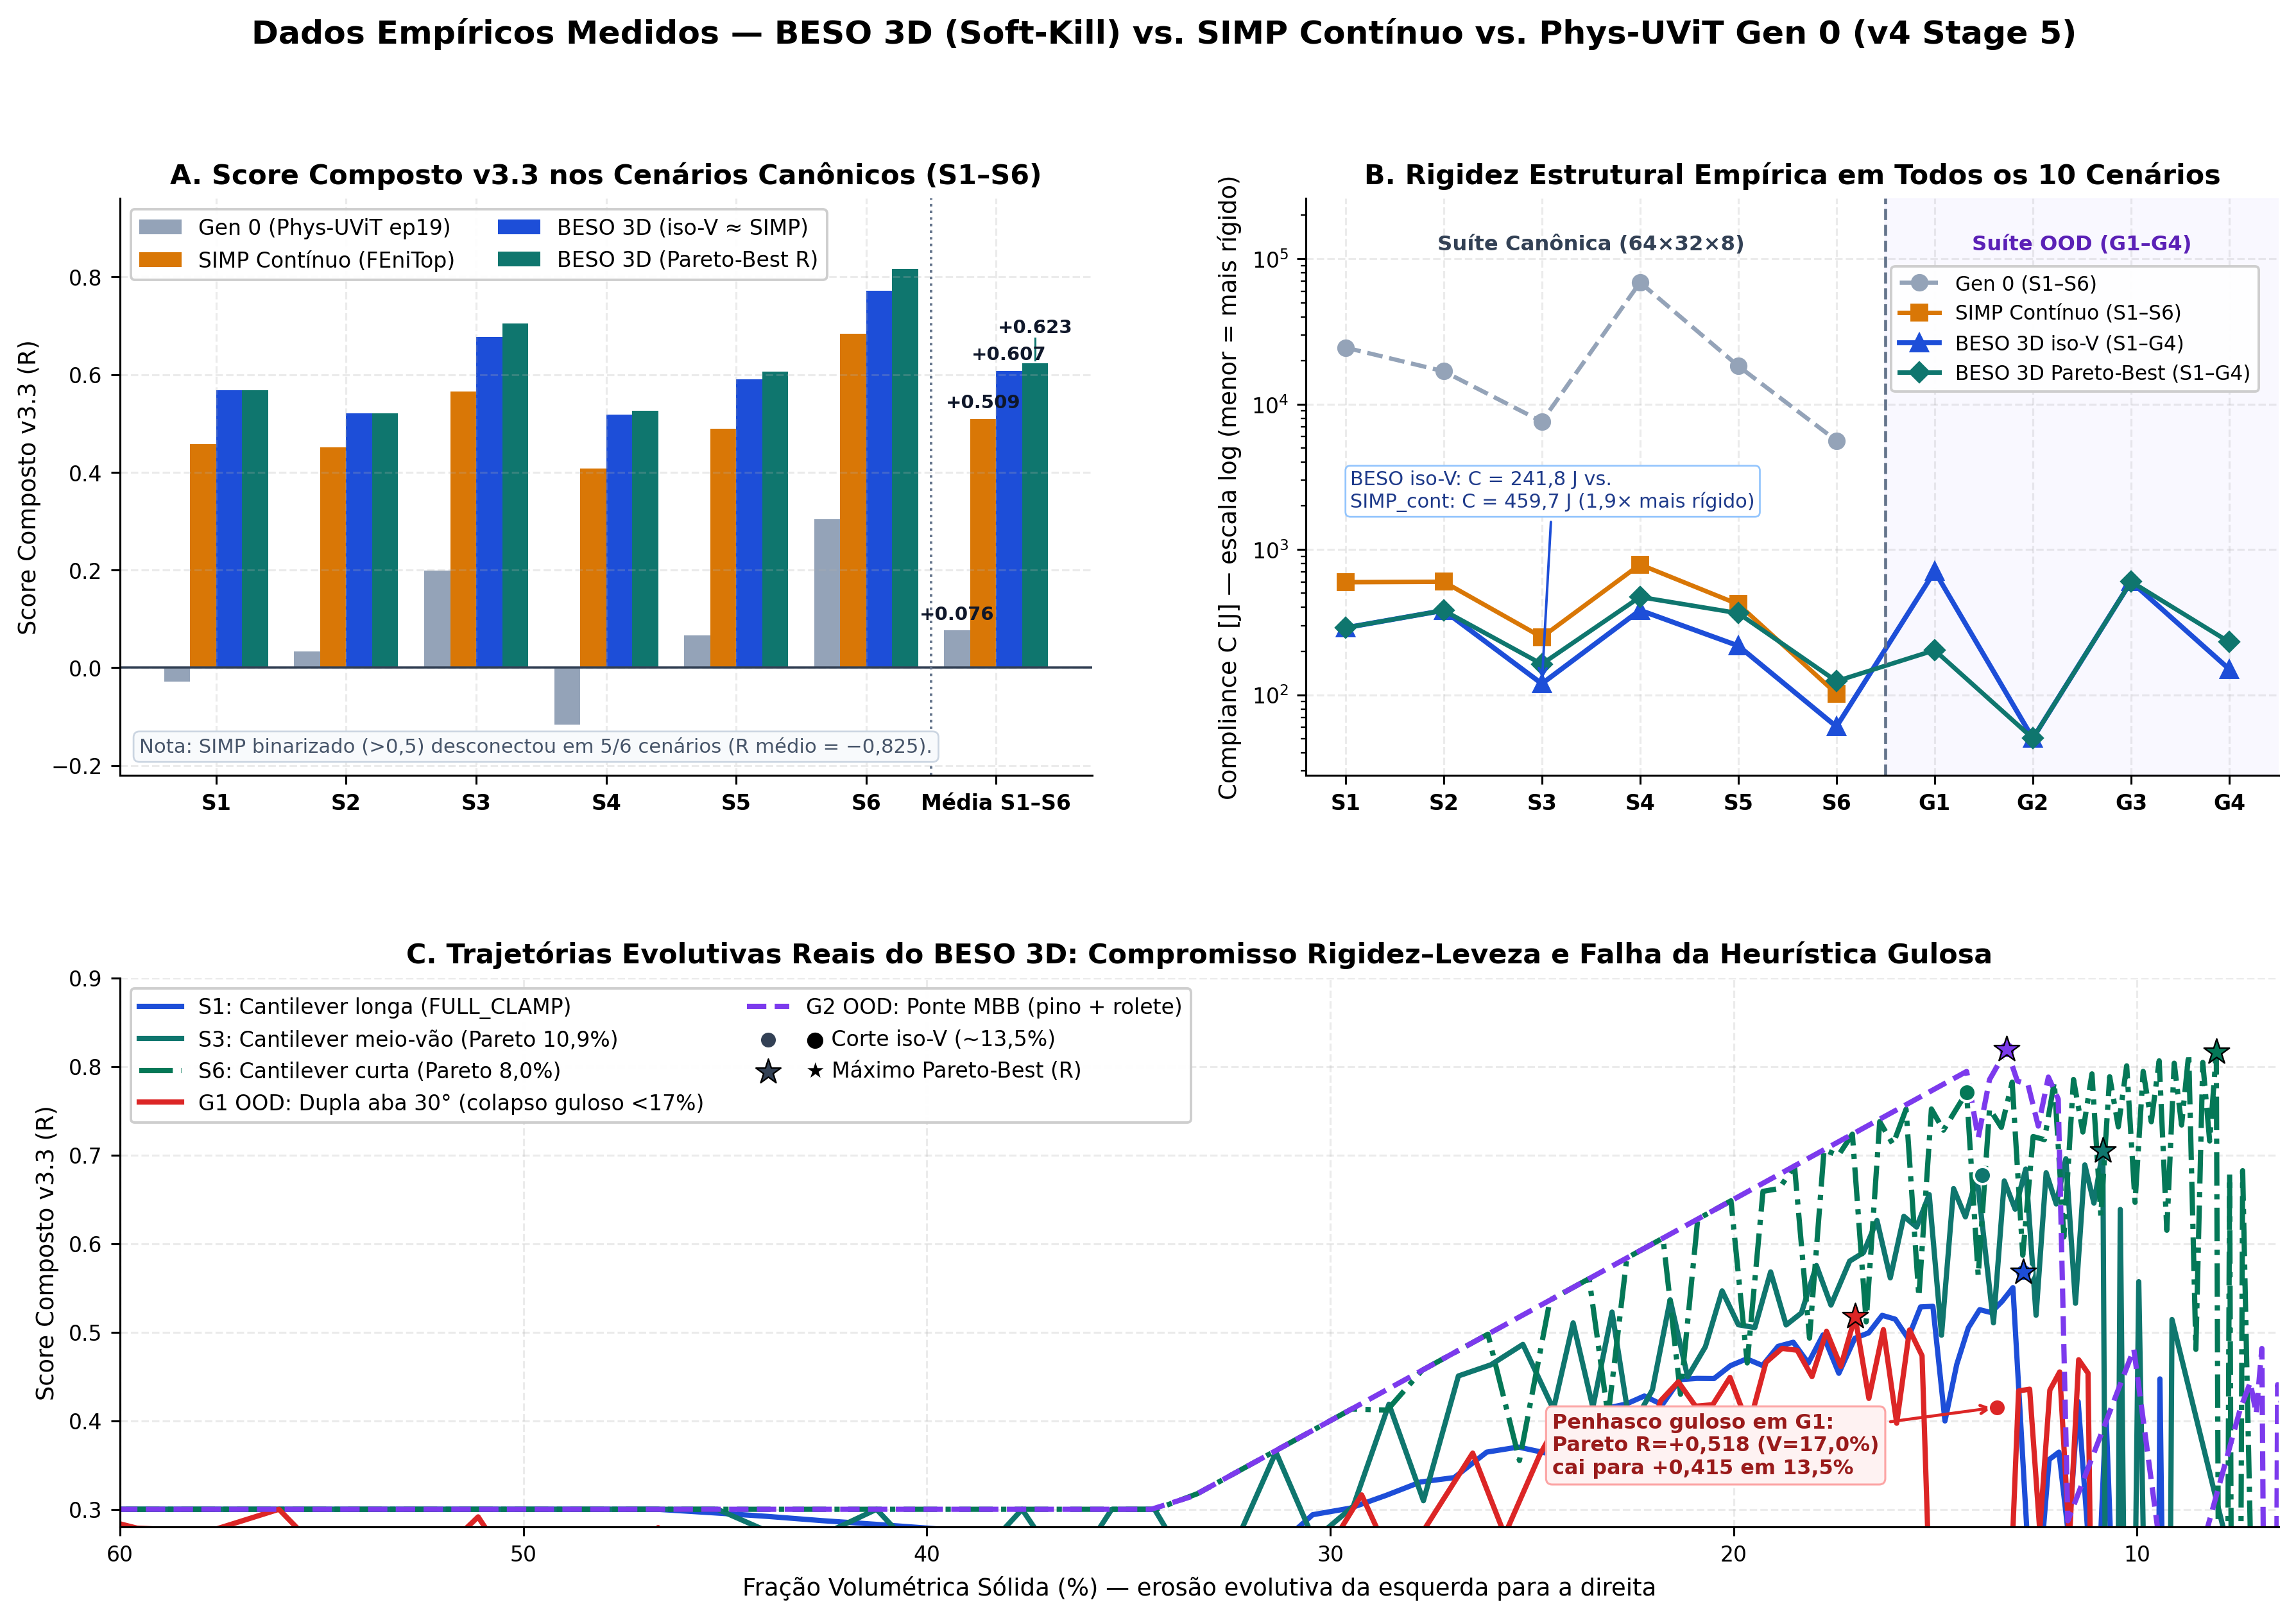
\includegraphics[width=0.98\linewidth]{fig_sota01_beso3d_vs_simp_vs_gen0.png}
  \caption{Desempenho empírico medido nos cenários canônicos (\texttt{S1}--\texttt{S6}) e OOD (\texttt{G1}--\texttt{G4}). O \texttt{SIMP\_bin} após corte discreto ($>0{,}5$) desconectou em 5 de 6 cenários ($R_{\text{médio}} = -0{,}8253$), enquanto o BESO 3D reduziu a compliance quase à metade frente ao \texttt{SIMP\_cont} em iso-volume ($241{,}8\text{ J}$ contra $459{,}7\text{ J}$). No Painel C, observa-se a queda gulosa de \texttt{G1} abaixo de $17\%$.}
  \label{fig:sota01}
\end{figure}

Quatro conclusões empíricas diretas emergem da Figura~\ref{fig:sota01} e da inspeção das geometrias reais da Figura~\ref{fig:sota02}:

\begin{itemize}
  \item \textbf{Superioridade binária real do BESO 3D sobre o \texttt{SIMP\_cont}:} Em volume equivalente ($13{,}45\%$ contra $13{,}51\%$), o BESO 3D atinge $+0{,}6074$ ($241{,}8\text{ J}$) ante $+0{,}5092$ ($459{,}7\text{ J}$) do SIMP contínuo, porque elimina densidades cinza penalizadas por $\rho^3$ e concentra toda a massa em barras binárias cheias com $54{,}67\%$ a $60{,}78\%$ de área projetada oca (\texttt{hol}).
  \item \textbf{O penhasco guloso em \texttt{G1}:} Em dupla aba com carga inclinada a $30^\circ$, o BESO atinge ótimo local $R = +0{,}5176$ com $16{,}99\%$ de volume ($203{,}0\text{ J}$), mas despenca abruptamente para $R = +0{,}4152$ ($708{,}9\text{ J}$) ao prosseguir erodindo até $13{,}48\%$ — evidência direta da falha de busca estritamente local e monotônica diante de apoios não convexos.
  \item \textbf{Aproveitamento genuíno do terceiro eixo em \texttt{S5}:} Na viga excêntrica em profundidade ($z \in [1, 3]$ sobre $Z \in [0, 7]$), o BESO posiciona o centroide longitudinal em $z_c = 2{,}575$ na solução Pareto-Best, gerando seção vazada assimétrica (Figura~\ref{fig:sota02}), em contraste com a viga fina de \texttt{Gen 0} ($\mathrm{hol} = 3{,}41\%$).
  \item \textbf{Custo de execução rígido e zero transferência:} O conjunto completo dos 10 cenários consumiu $1\,680{,}8\text{ s}$ de parede com 4 trabalhadores paralelos, exigindo $6{,}34\text{ s}$ por iteração FEM e $83$ a $115$ chamadas completas de FEM por estrutura, sem reaproveitar qualquer padrão estrutural para a peça seguinte.
\end{itemize}

\begin{figure}[htbp]
  \centering
  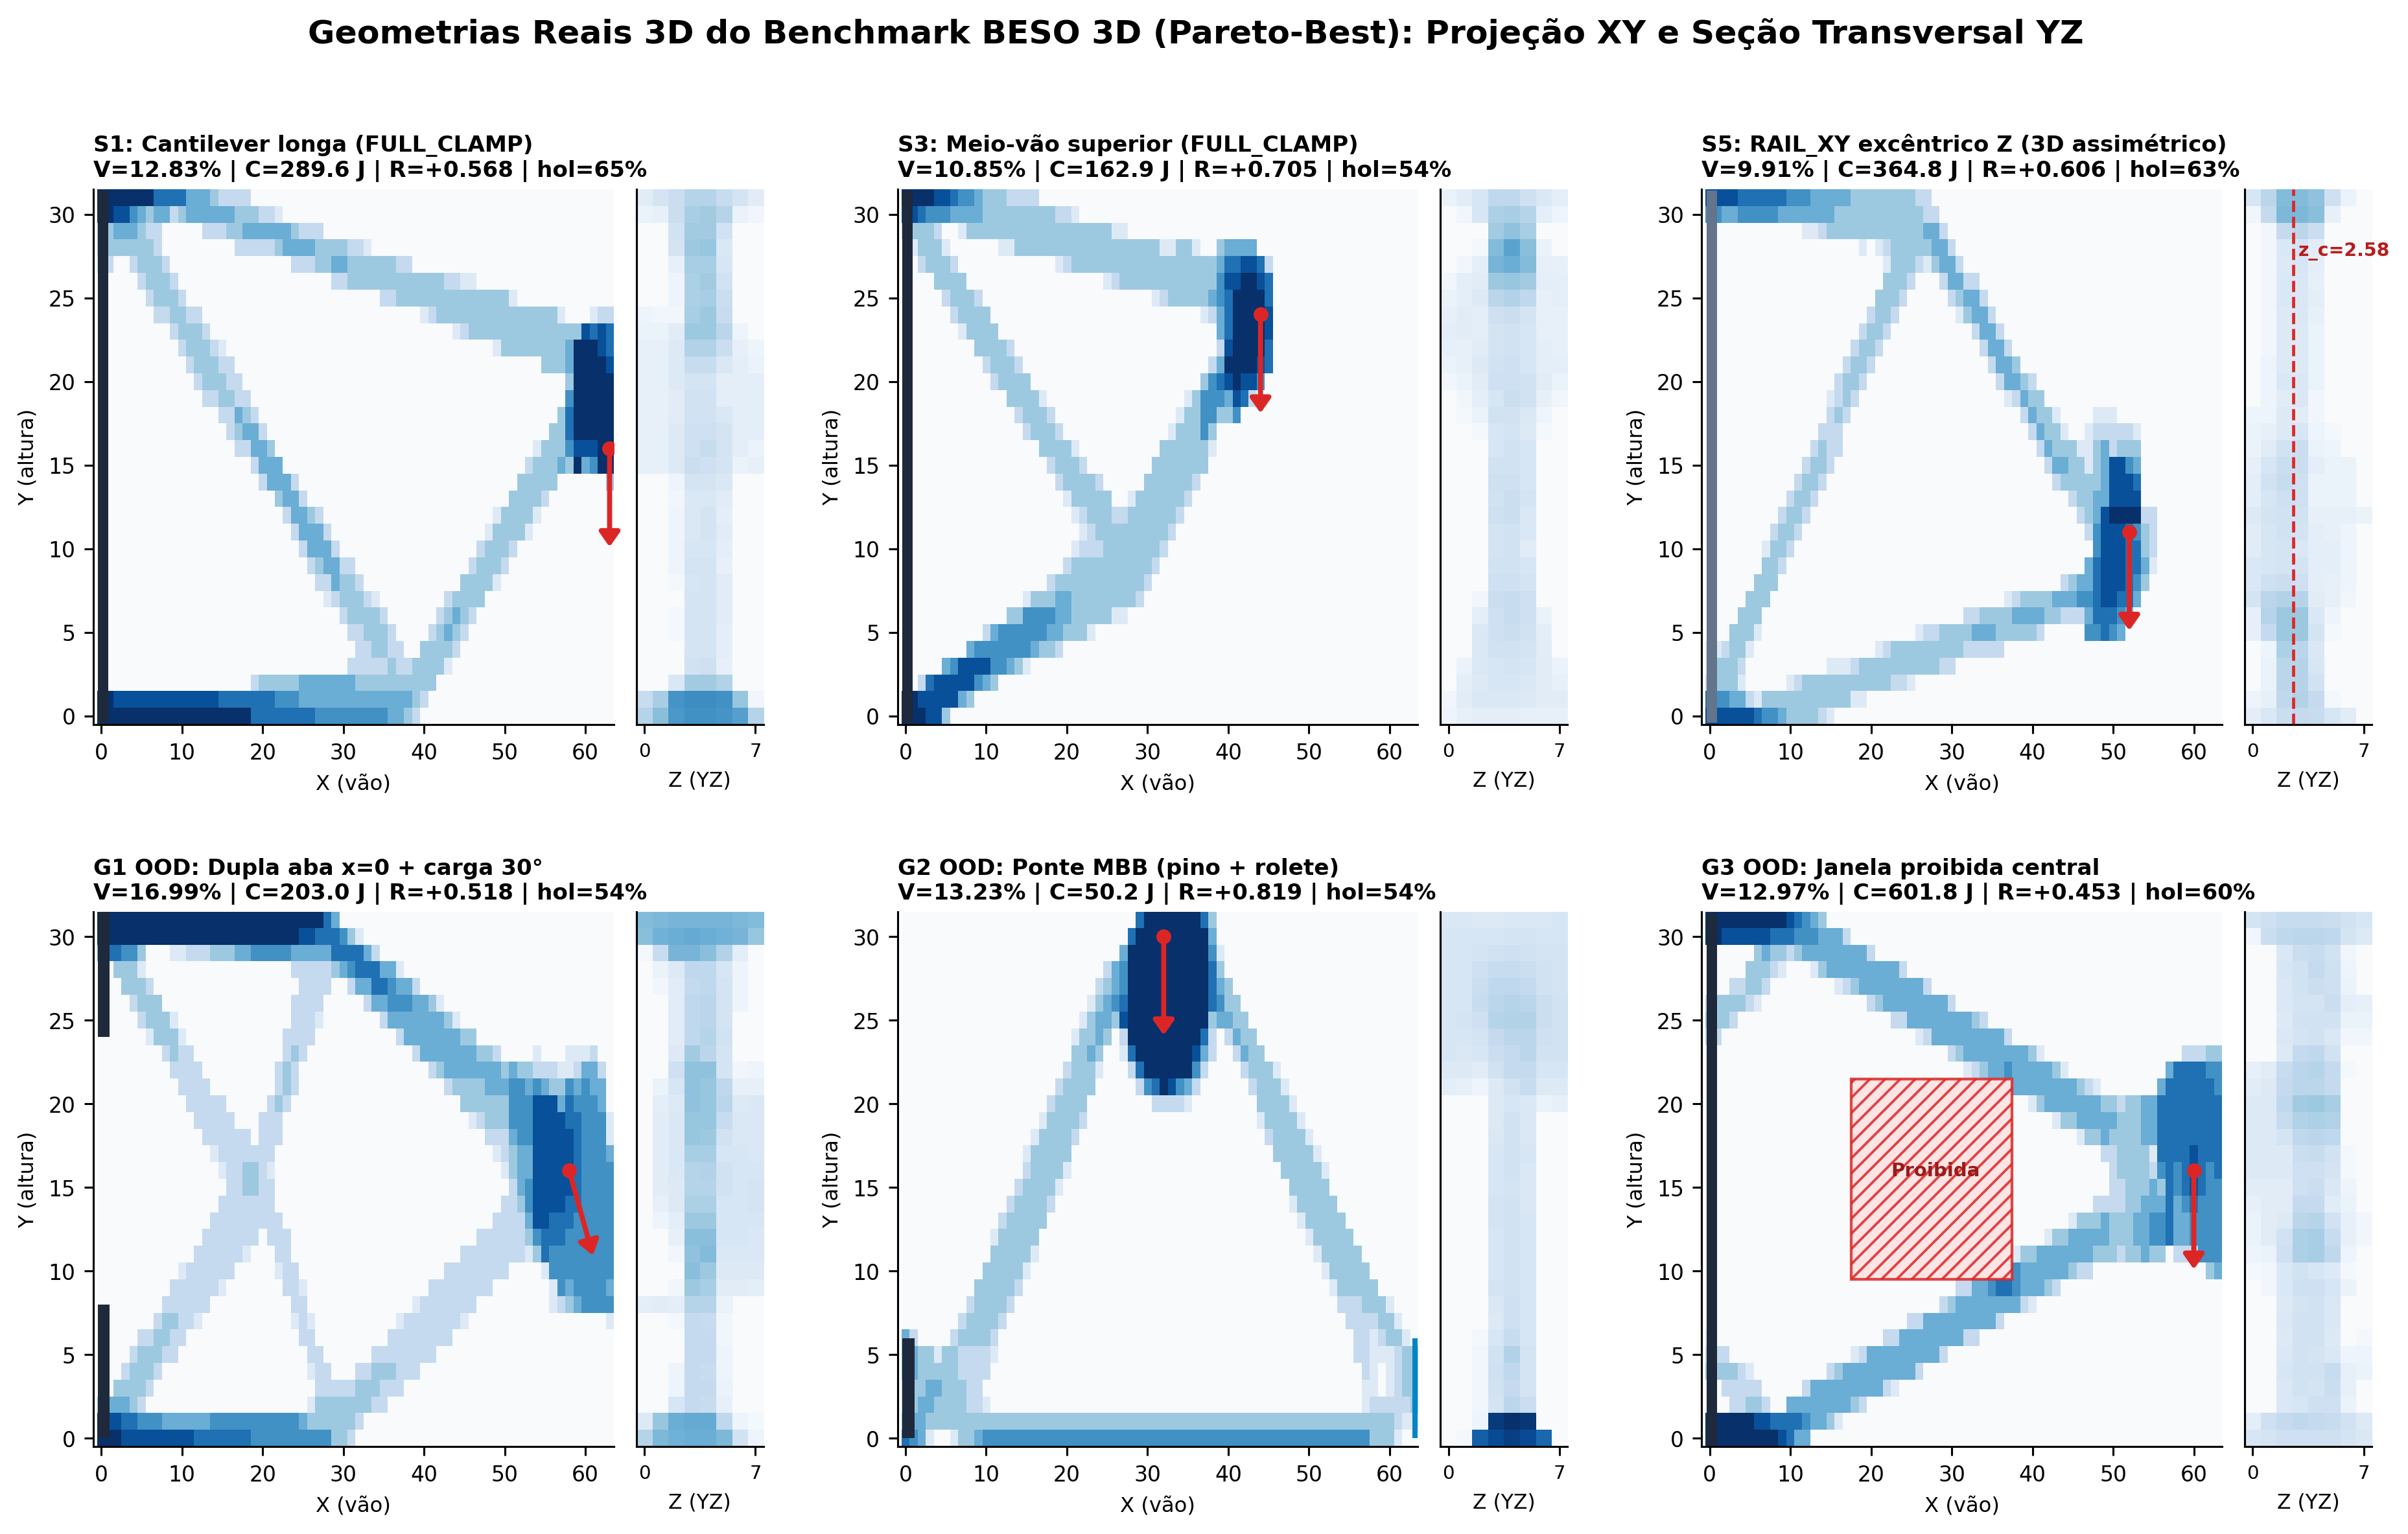
\includegraphics[width=0.98\linewidth]{fig_sota02_beso3d_real_geometries.png}
  \caption{Geometrias 3D reais obtidas pelo BESO 3D no ponto \texttt{Pareto-Best} em seis cenários representativos (projeção média em $Z$ no plano $XY$ acompanhada do corte transversal $YZ$ à direita). Em \texttt{S5}, destaca-se o deslocamento do centroide para $z_c = 2{,}58$ acompanhando o plano da carga.}
  \label{fig:sota02}
\end{figure}

% ==============================================================================
\section{Parte II --- Reforma Arquitetural do Buscador: \texttt{MCTS-DAG v4.1} e Preservação de Checkpoint}
\sectionmark{Parte II --- Reforma MCTS-DAG v4.1 e Checkpoint}
% ==============================================================================

A avaliação empírica do checkpoint \texttt{v4\_stage5} (\textbf{Gen 0}) revelou uma disfunção severa na Fase 2: ao longo dos seis cenários canônicos, o buscador executou $1\,435$ ações \texttt{ADD} contra apenas $5$ ações \texttt{REMOVE} ($99{,}65\%$ contra $0{,}35\%$), estagnando com fração volumétrica de $7{,}67\%$, compliance média de $23\,646\text{ J}$ e fração oca próxima de zero ($3{,}41\%$). Em vez de culpar apenas o pré-treino neural, a auditoria algorítmica demonstrou cinco gargalos estruturais no algoritmo de busca em árvore de Monte Carlo (\textbf{MCTS}, \textit{Monte Carlo Tree Search}) que impediam qualquer rede — mesmo perfeitamente treinada — de esculpir treliças vazadas. Todos foram corrigidos na arquitetura \texttt{MCTS-DAG v4.1}.

\begin{figure}[htbp]
  \centering
  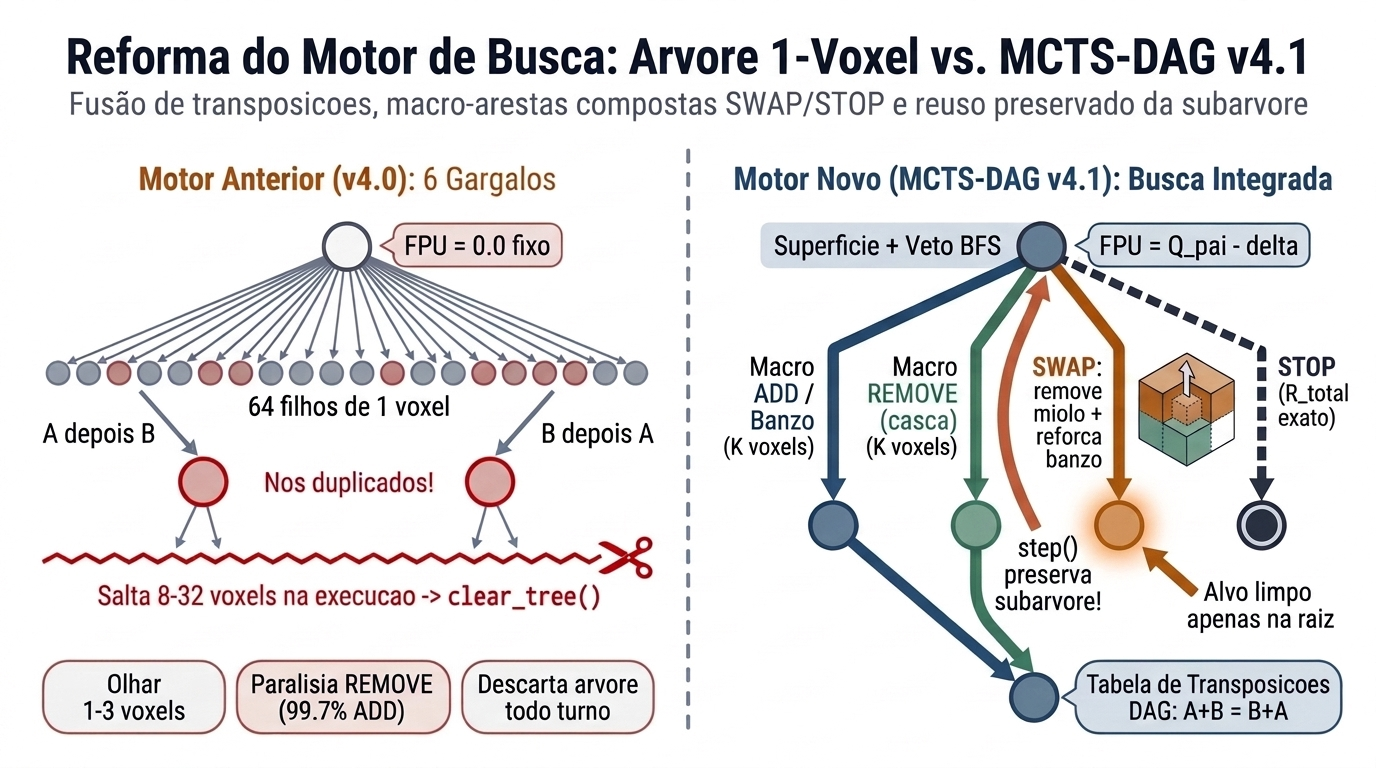
\includegraphics[width=0.98\linewidth]{diag02_mcts_v41_dag_macro_swap.jpg}
  \caption{Arquitetura comparativa entre o motor anterior de 1 voxel (\texttt{v4.0}, à esquerda) e o buscador \texttt{MCTS-DAG v4.1} integrado com filtro de superfície, veto BFS, macro-ações compostas \texttt{SWAP}/\texttt{STOP}, tabela de transposições e reuso da subárvore (\texttt{step()}).}
  \label{fig:diag02}
\end{figure}

\subsection{As Cinco Atualizações do Motor de Busca}

Em otimização sequencial guiada por valor e política, a pontuação de seleção de cada candidato segue o critério \textbf{PUCT} (\textit{Predictor Upper Confidence bound applied to Trees}) \cite{kocsis2006bandit, rosin2011multi, silver2017mastering}:
\begin{equation}
  \mathrm{PUCT}(s, a) = Q(s, a) + c_{\mathrm{puct}}\, P(s, a)\, \frac{\sqrt{N_{\mathrm{pai}}}}{1 + N(s, a) + N_{\mathrm{vl}}(s, a)}
  \label{eq:puct}
\end{equation}
em que $P(s, a)$ é a probabilidade a priori fornecida pela rede neural, $N_{\mathrm{pai}}$ é o total de visitas no estado pai e $N_{\mathrm{vl}}$ é a \textbf{perda virtual} (\textit{virtual loss}), penalização provisória aplicada durante simulações em lote para evitar que todas as consultas simultâneas percorram o mesmo caminho. A reforma da versão \texttt{v4.1} atua sobre cinco eixos acoplados em \texttt{alphabuilder/src/logic/mcts/\{legal\_moves.py, node.py, engine.py\}}:

\begin{enumerate}
  \item \textbf{FPU Relativo ao Nó Pai e Desempate na Simulação Inicial:} Um nó candidato ainda não visitado ($N = 0$) não possui média empírica $Q$, exigindo um valor inicial assumido denominado \textbf{FPU} (\textit{First Play Urgency}, urgência da primeira jogada) \cite{browne2012survey, wu2019accelerating}. O motor antigo adotava $\mathrm{FPU} = 0{,}0$ fixo. Quando uma estrutura conectada já alcançava $Q_{\mathrm{pai}} = +0{,}45$, um ramo não visitado de escavação (\texttt{REMOVE}) sofria punição implícita de $-0{,}45$ em relação ao pai, permanecendo inexplorado frente a irmãos \texttt{ADD} já visitados. Na \texttt{v4.1}, \texttt{select\_child} substitui o valor nulo pelo FPU relativo $\mathrm{FPU} = \max(-1{,}0, Q_{\mathrm{pai}} - \delta_{\mathrm{fpu}})$, com $\delta_{\mathrm{fpu}} = 0{,}20$ na Fase 1 (\texttt{PHASE1\_V41\_CONFIG}) e $0{,}25$ na Fase 2 (\texttt{PHASE2\_V41\_CONFIG}). Ademais, \texttt{parent\_eff = max(1, total\_visits)} garante quebra determinística de empates pelo prior $P(s,a)$ na primeira iteração ($N_{\mathrm{pai}} = 0$) ou sob perda virtual ativa.

  \item \textbf{Remoção Restrita à Superfície Exposta e Veto BFS em Lote:} Retirar voxels no miolo maciço cria poros internos fechados sem alívio de tensão útil ou fragmenta barras esbeltas. Com \texttt{surface\_only\_remove=True}, \texttt{get\_legal\_remove\_moves} filtra candidatos \texttt{REMOVE} apenas na interface sólido--vazio (6-conectividade). Durante a aplicação efetiva do lote escolhido, \texttt{filter\_disconnect\_safe\_batch} executa uma busca em largura (\textbf{BFS}, \textit{Breadth-First Search}, varredura por camadas no grafo de adjacência 3D) após cada voxel candidato: caso aquele voxel seja um \textit{ponto de articulação} cuja remoção rompa a continuidade entre suporte e carga ou multiplique ilhas soltas, o movimento é vetado instantaneamente antes de invocar o FEM.

  \item \textbf{Alvo Limpo de Política na Raiz (\texttt{get\_root\_voxel\_visits}):} Anteriormente, a função \texttt{collect\_subtree\_visits} acumulava contagens de visitas de nós em profundidade $d = 2\text{--}4$ dentro do vetor-alvo de treinamento da raiz $d = 0$, contaminando o gradiente de política \cite{huang2022closer} com coordenadas ainda ilegais na geometria inicial. Com \texttt{root\_only\_policy\_target=True}, o alvo empírico passa a projetar estritamente os filhos diretos da raiz ($\pi_{\mathrm{MCTS}}$ limpo).

  \item \textbf{Macro-Ações Compostas (\texttt{ADD}/\texttt{REMOVE}/\texttt{SWAP}/\texttt{STOP}) e Reuso da Subárvore:} Na versão \texttt{v4.0}, o buscador simulava edições de 1 único voxel, mas executava saltos de 8 a 32 voxels e descartava a árvore inteira com \texttt{clear\_tree()} em seguida. Agora, \texttt{expand\_macro} gera até $14$ (Fase 1) ou $16$ (Fase 2) macro-arestas contendo exatamente os blocos de até $K$ voxels alinhados aos passos reais do ambiente: blocos \texttt{ADD} nos banzos tracionados/comprimidos, blocos \texttt{REMOVE} de escavação de alma, movimentos compostos \textbf{\texttt{SWAP}} conservadores de massa (remove voxels neutros de superfície e adiciona imediatamente na fibra extrema, impossível de formular em edições de 1 voxel sem violar volume intermediário) e a ação terminal voluntária \textbf{\texttt{STOP}}. Como a transição do episódio coincide com uma aresta real da raiz, \texttt{mcts.step(macro\_act)} desloca o ponteiro da raiz preservando toda a subárvore já explorada.

  \item \textbf{Tabela de Transposições \texttt{MCTS-DAG}, Crescimento Bidirecional e Política Fatorada:} Em otimização estática de voxels, adicionar ou remover $A$ e depois $B$ produz exatamente a mesma configuração binária que aplicar $B$ e depois $A$. Uma árvore convencional duplica esses nós $d!$ vezes. Com \texttt{use\_transposition\_dag=True}, \texttt{compute\_state\_hash} (hash MD5 da malha binária, fase e assinaturas de carga/apoio) funde estados equivalentes em um grafo acíclico dirigido (\textbf{DAG}, \textit{Directed Acyclic Graph}) protegido contra ciclos (\texttt{id(existing) not in ancestor\_ids}), concentrando todas as estatísticas na mesma representação física. Na Fase 1, \texttt{bidirectional\_p1=True} habilita sementes tanto no engaste quanto na região de carga (\texttt{include\_load\_seeds=True}), acelerando drasticamente o encontro de pontes e reduzindo o risco de desvio para o infinito.
\end{enumerate}

\subsection{Preservação Bit-a-Bit do Checkpoint \texttt{v4\_stage5} via \texttt{op\_head} Zero-Inicializada}

Uma preocupação prática legítima diante de qualquer mudança arquitetural na rede neural (\textit{policy} + \textit{value network}) é saber se o investimento de pré-treino acumulado no checkpoint \texttt{phys\_uvit\_v4\_stage5\_best.pt} (\textbf{checkpoint}, fotografia completa dos pesos sinápticos da rede neural salva em disco) se perde ao introduzir novas operações como \texttt{STOP} e \texttt{SWAP}. A resposta é categórica: \textbf{nenhum peso pré-treinado se perde}.

Para corrigir o desequilíbrio estrutural de probabilidades entre $N_{\mathrm{add}} \gg N_{\mathrm{rem}}$ e dotar o agente de decisão de encerramento, adicionamos à classe \texttt{PhysUViT3D} (\texttt{alphabuilder/\allowbreak{}src/\allowbreak{}neural/\allowbreak{}phys\_uvit.py}) uma cabeça linear enxuta responsável pela distribuição de probabilidade global sobre o tipo de operação [\texttt{ADD}, \texttt{REMOVE}, \texttt{STOP}]:
\begin{equation}
  \mathbf{z}_{\mathrm{op}} = \texttt{op\_head}\big([\mathbf{h}_{\mathrm{global}} \,\|\, \mathbf{h}_{\mathrm{phys}}]\big) \in \mathbb{R}^3, \quad \texttt{Linear}(384 \to 3)
\end{equation}
Adicionando apenas \textbf{$1\,155$ parâmetros} aos $4\,912\,683$ parâmetros da base Stage 6 com cabeça física auxiliar (\texttt{sed\_head}, frente a $4\,884\,839$ da base Stage 5 original), o modelo totaliza \textbf{$4\,913\,838$ parâmetros}. Como \texttt{op\_head} é inicializada com pesos e viés rigorosamente em zero (\texttt{weight.zero\_()}, \texttt{bias.zero\_()}) e os módulos \texttt{inference.py} e \texttt{train\_selfplay\_step.py} carregam checkpoints via \texttt{strict=False} com validação de lista branca (\textit{whitelist} verificando que apenas chaves \texttt{op\_head.*} podem faltar), no passo zero vale exatamente $\mathrm{softmax}([0,0,0]) = (1/3, 1/3, 1/3)$ — testado explicitamente com tolerância de $10^{-4}$ na suíte unitária. Todas as representações espaciais do \textit{Transformer} 3D, do decodificador U-Net, do valor $V$ e do estimador auxiliar de energia de deformação permanecem $100\%$ intactas desde a primeira iteração de auto-jogo.

% ==============================================================================
\section{Parte III --- Blindagem do Ciclo de Vida: Progressão, Transição e Encerramento}
\sectionmark{Parte III --- Blindagem do Ciclo de Vida}
% ==============================================================================

Em aprendizado por reforço sequencial acoplado a um simulador físico, a rede aprende estritamente a partir dos alvos gravados ao fim de cada episódio. Se a transição entre fases matar estruturas promissoras no instante errado ou se o sinal de retropropagação atribuir notas ruins a estados intermediários ótimos apenas por degeneração tardia, o ciclo inteiro diverge. A Figura~\ref{fig:diag03} sintetiza as sete correções de ciclo de vida integradas nos arquivos \texttt{reward.py}, \texttt{storage.py} e \texttt{runner.py}.

\begin{figure}[htbp]
  \centering
  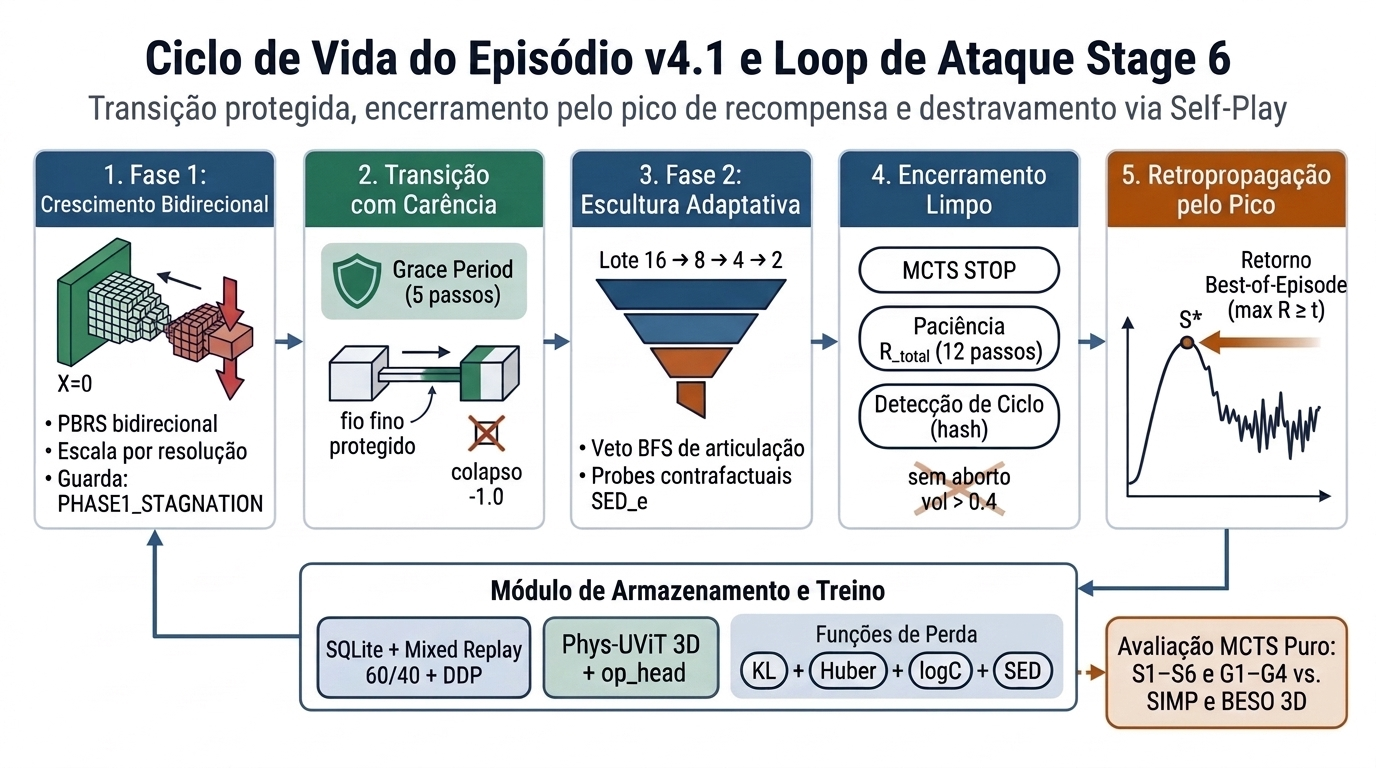
\includegraphics[width=0.98\linewidth]{diag03_phase_lifecycle_and_attack_pipeline.jpg}
  \caption{Ciclo de vida completo do episódio na versão \texttt{v4.1} (acima) integrado ao ciclo iterativo de treinamento Stage 6 com banco SQLite, \textit{replay buffer} misto e avaliação determinística dupla.}
  \label{fig:diag03}
\end{figure}

\subsection{As Sete Blindagens da Progressão, Transição e Encerramento}

\begin{enumerate}
  \item \textbf{Remoção do Aborto Prematuro em \texttt{vol > 0.40} (\texttt{reward.py}):} A condição de parada terminal por excesso de massa em \texttt{get\_phase2\_terminal\_reward} interrompia o episódio assim que $V > 0{,}40$, impedindo trajetórias espessas iniciais que posteriormente se refinam com segurança para $10\%\text{--}13\%$ (como ocorre naturalmente no BESO). O teto foi elevado para \texttt{max\_vol\_frac = 0{,}65}.
  \item \textbf{Período de Carência Pós-Conexão (\textit{Grace Period}, \texttt{p2\_grace\_steps = 5}):} Assim que a Fase 1 fecha o primeiro caminho ligando suporte e carga, a ponte recém-formada costuma ter 1 a 2 voxels de seção e deslocamento bruto acima de $u_{\mathrm{lim}} = 128\,000$ \cite{hayashi2020reinforcement}. Sem carência, o primeiro cálculo de FEM reprovava o episódio instantaneamente com recompensa $-1{,}0$. Nos 5 primeiros passos de Fase 2, \texttt{calculate\_grace\_displacement\_reward} substitui a morte súbita por uma penalidade suave logarítmica limitada a $[-0{,}98; -0{,}85]$, preservando o episódio vivo e dando sinal de gradiente para o MCTS engrossar os banzos críticos antes da ativação do critério rígido de colapso.
  \item \textbf{Parada por Paciência em $R_{\mathrm{total}}$, Detecção de Ciclos e \texttt{MCTS\_STOP}:} A convergência antiga monitorava apenas variação de compliance isolada. Agora, a Fase 2 encerra por três vias fisicamente coerentes: (a) seleção voluntária de \texttt{MCTS\_STOP} a partir do passo $6$ da Fase 2 (\texttt{p2\_min\_stop\_steps = 6}); (b) esgotamento de paciência de $12$ passos sem melhoria no máximo global $R_{\mathrm{total}}$ (\texttt{p2\_patience = 12}, motivo \texttt{REWARD\_CONVERGENCE}); ou (c) detecção de estado binário idêntico repetido via hash MD5 (\texttt{CYCLE\_DETECTED}), impedindo oscilações infinitas \texttt{ADD/REMOVE}.
  \item \textbf{Retropropagação Protegida pelo Pico (\textit{Best-of-Episode}, \texttt{storage.py}):} Anteriormente, um episódio que atingia um pico brilhante $R^* = +0{,}71$ no passo $14$ mas continuava erodindo até cair para $+0{,}38$ no passo $28$ tinha todos os seus estados anteriores retroalimentados pelo último valor degenerado. Com \texttt{use\_best\_of\_episode\_targets=True} e mantendo consistência exata da penalidade de ilhas ($R_{\mathrm{total}}(\tau) = R_{\mathrm{fem}}(\tau) - P_{\mathrm{island}}(\tau)$), o alvo de treinamento da cabeça de valor para todo passo $t$ passa a ser:
  \begin{equation}
    z_t = \max_{\tau \ge t} \left[ R_{\mathrm{total}}(\tau)\,\gamma^{\tau - t} \right], \qquad \gamma = 0{,}99
    \label{eq:best_of_ep}
  \end{equation}
  Dessa forma, o trecho de construção até o ótimo recebe integralmente o sinal positivo de sucesso, enquanto os passos degenerados após $t^*$ carregam retorno decrescente, ensinando \texttt{op\_head} a acionar \texttt{STOP} exatamente ao cruzar o cume da trajetória.
  \item \textbf{Escala de Lote por Resolução na Fase 1 e Guarda de Estagnação:} O tamanho de lote na Fase 1 escala com $(N / 16\,384)^{1/3}$, evitando passos gigantescos em domínios compactos como $48\times 24\times 12$, enquanto \texttt{p1\_stagnation\_patience = 20} aborta episódios travados (\texttt{PHASE1\_STAGNATION}) sem consumir cota desnecessária.
  \item \textbf{Cronograma Adaptativo Grosseiro-para-Fino na Fase 2 (\texttt{p2\_batch\_schedule = (16, 8, 4, 2)}):} Passos iniciais amplos ($16$ e $8$ voxels) modelam rapidamente as grandes cavidades de alma e banzos, reduzindo-se progressivamente para $4$ e $2$ voxels no ajuste fino próximo ao ótimo de Pareto, complementados por \textit{probes} contrafactuais de densidade de energia de deformação (\textbf{SED}, \textit{Strain Energy Density}) para alimentar exemplos contrastivos no banco de replay \cite{wang2020warmstart, nakamoto2023calql}.
  \item \textbf{Restauração da Fase 1 em \texttt{resume\_episode}:} Corrigida a lógica de retomada em episódios gravados parcialmente no SQLite para restabelecer corretamente contadores e estado da Fase 1 antes de atingir conectividade.
\end{enumerate}

\begin{figure}[htbp]
  \centering
  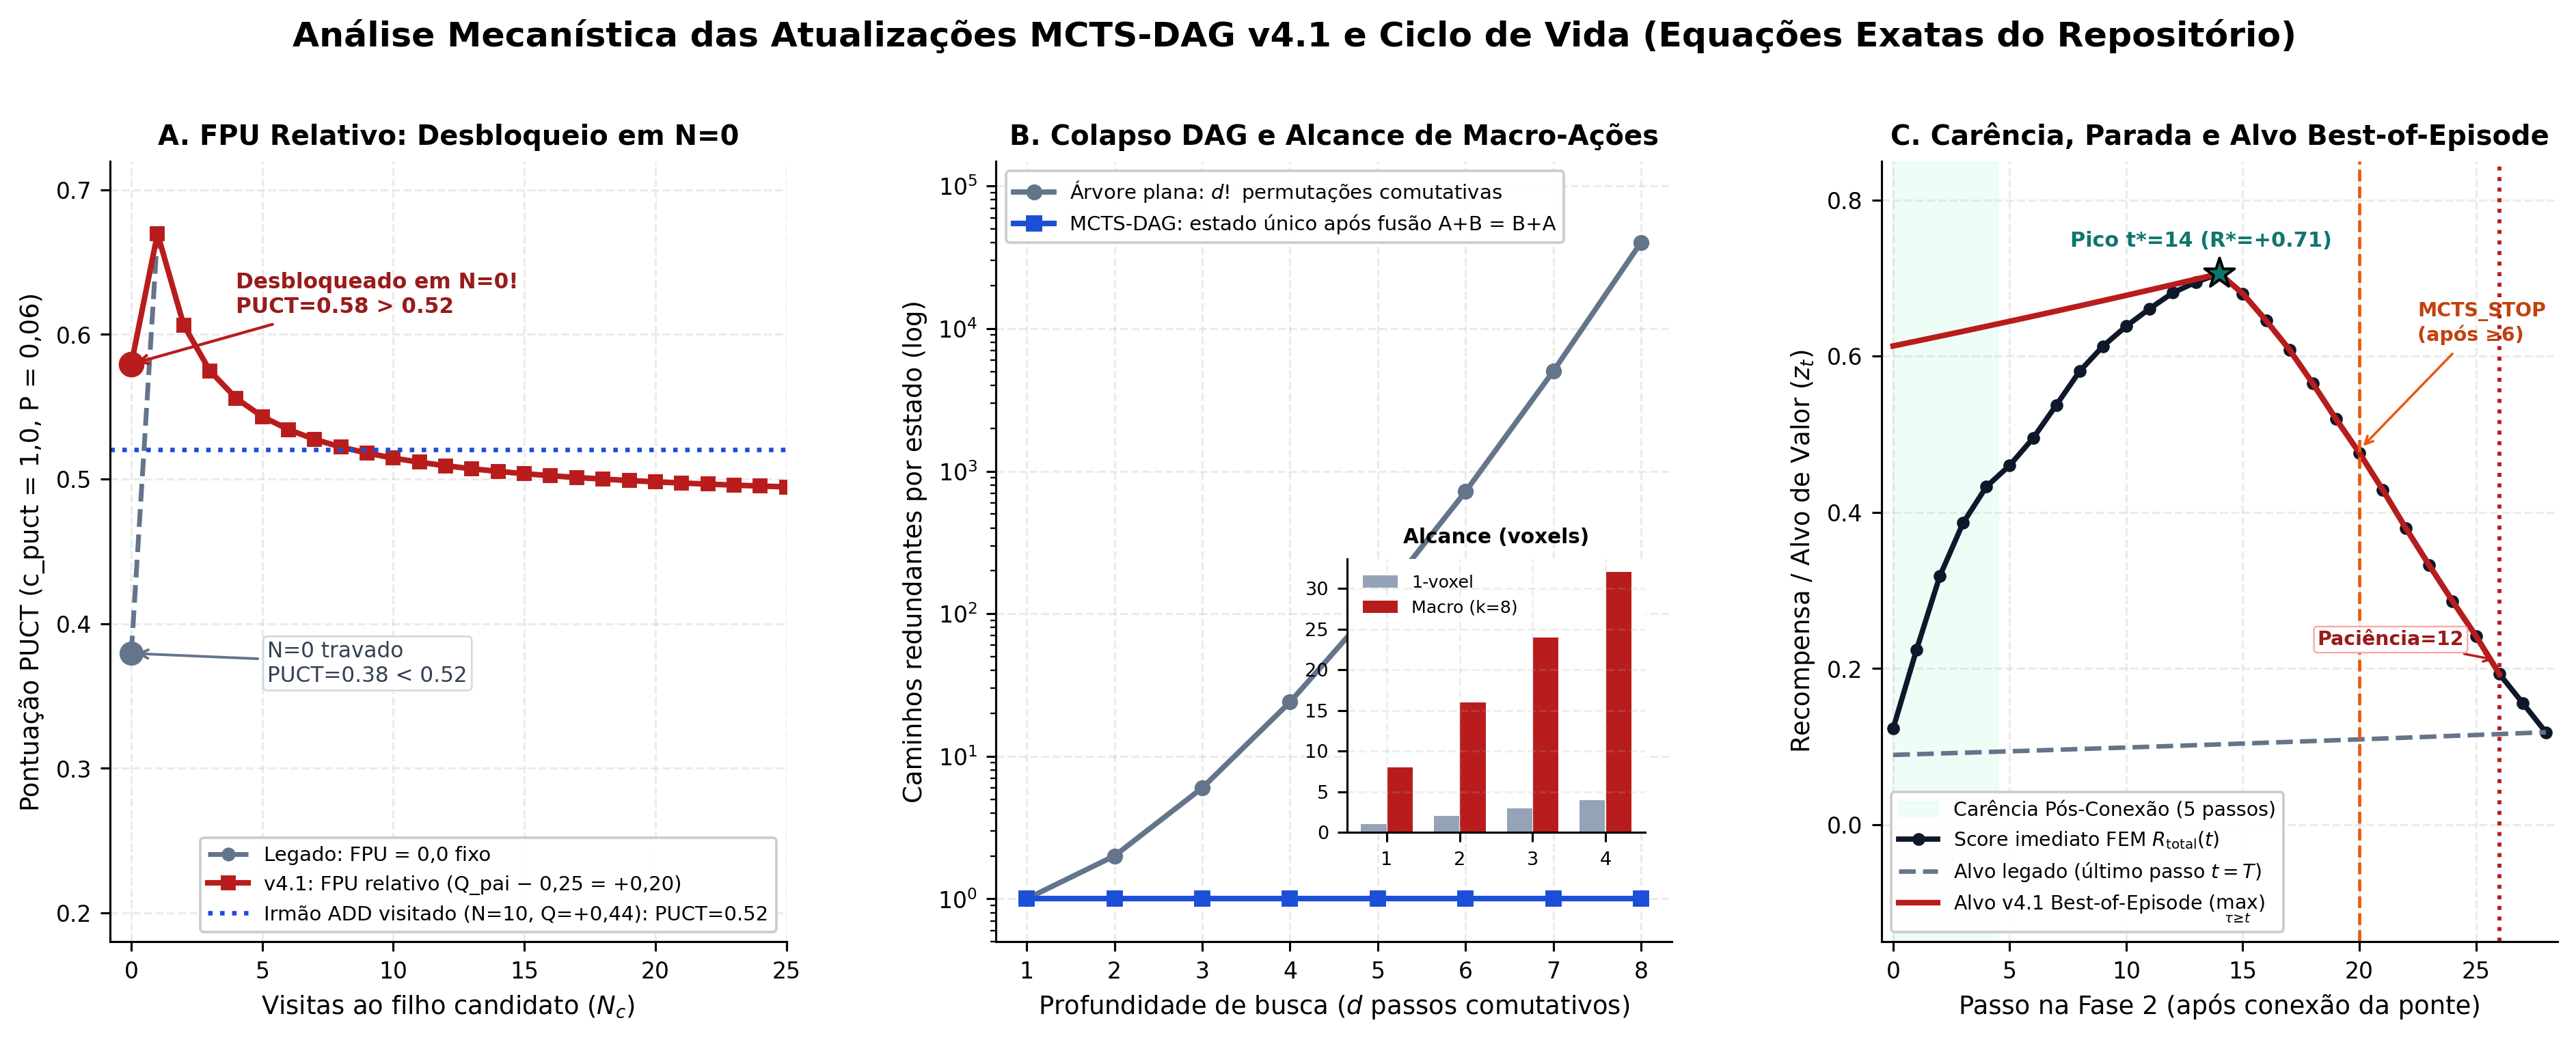
\includegraphics[width=0.98\linewidth]{fig_sota03_mcts_and_termination_ablation.png}
  \caption{Análise mecanística exata sob as equações do repositório: (A) desbloqueio de ações \texttt{REMOVE}/\texttt{SWAP} não visitadas pelo FPU relativo frente à paralisia de $\mathrm{FPU}=0$; (B) colapso das $d!$ trajetórias comutativas no \texttt{MCTS-DAG} e ganho de horizonte $8\times$ das macro-ações; (C) proteção pela carência pós-conexão, parada por paciência/\texttt{STOP} e alvos descontados \textit{best-of-episode}.}
  \label{fig:sota03}
\end{figure}

% ==============================================================================
\section{Parte IV --- Preparação Pré-Self-Play e Protocolo Operacional da Etapa 6}
\sectionmark{Parte IV --- Protocolo Operacional Etapa 6}
% ==============================================================================

A execução de auto-jogo com simulações FEM reais em GPU deve ocorrer somente após esgotar todas as verificações determinísticas em CPU e isolar os ganhos puramente algorítmicos. Esta seção fixa o protocolo exato a ser cumprido antes e durante a campanha iterativa.

\subsection{Lista de Prontidão Pré-Auto-Jogo}

\begin{enumerate}
  \item \textbf{Auditoria da Suíte Unitária (Concluída em CPU):} Após todas as edições da revisão \texttt{v4.1} e do módulo \texttt{BESO 3D}, a suíte completa em \texttt{pytest tests/unit/ -v} encerrou com \textbf{$156$ testes aprovados, $0$ falhas e $1$ teste MPI pulado} (\texttt{test\_run\_fenitop\_optimization}), validando desde o ordenamento de perda virtual até simulações completas de ponta a ponta no \texttt{runner.py} e convergência do \texttt{beso3d.py}.
  \item \textbf{Benchmarking de Paridade Física (Concluída):} Discrepância máxima verificada de $1{,}95 \times 10^{-8}$ entre \texttt{fast\_amg} e \texttt{DOLFINx}, assegurando que nenhum ganho futuro venha de erro de discretização ou de solver.
  \item \textbf{Ablação Zero-Retrain no Início da Sessão GPU (\texttt{Gen 0 + v4.1}):} Antes de disparar a Geração 1 de treinamento, executar \texttt{scripts/evaluate\_inference\_scenarios.py --v41-mcts} sobre o checkpoint atual \texttt{phys\_uvit\_v4\_stage5\_best.pt} ($\approx 20\text{ min}$ em T4). Essa leitura quantifica exatamente o salto isolado produzido pelo motor \texttt{MCTS-DAG v4.1} antes de atualizar um único peso sináptico.
\end{enumerate}

\subsection{Arquitetura de Treinamento Incremental, Currículo e Telemetria}

A cada geração $g \ge 1$ conduzida por \texttt{scripts/run\_selfplay\_pipeline.py} (em modo padrão \texttt{v4.1}, preservando \texttt{--legacy-mcts} como controle regressivo) e orquestrada pelo notebook \texttt{notebooks/alphabuilder-v4-stage6-selfplay.ipynb}, operam quatro mecanismos coordenados:

\begin{itemize}
  \item \textbf{Currículo em 4 Anéis Físicos (\texttt{scenarios\_stage6.py}):} A distribuição de cenários progride de \texttt{Tier 0} (cantilevers \texttt{FULL\_CLAMP} e \texttt{RAIL\_XY} com exclusão estrita da vizinhança dos testes \texttt{S1}--\texttt{S6} via \texttt{is\_near\_canonical\_scenario}), passando por \texttt{Tier 1} (abas duplas/parciais, cargas 3D inclinadas e cargas duplas), \texttt{Tier 2} (pontes MBB, apoios em L e janelas proibidas em \texttt{domain\_mask}), até \texttt{Tier 3} multi-resolução ($48\times 32\times 8$, $64\times 24\times 8$, $48\times 24\times 12$) explorando a invariância de escala da codificação posicional 3D (\textit{3D RoPE}) sem preenchimento com zeros (\textit{zero-padding}). Caso a taxa de conexão na Fase 1 de algum tier caia abaixo de $65\%$, \texttt{adjust\_tier\_weights} reduz automaticamente o peso dos níveis superiores.
  \item \textbf{Banco de Replay Misto 60/40 (\texttt{MixedReplayDataset}):} Cada época combina $60\%$ de trajetórias novas geradas por auto-jogo real e $40\%$ de amostras do banco de aquecimento supervisado (\texttt{warmup\_v3\_3\_kaggle.db}), estabilizando a distribuição física e evitando esquecimento catastrófico \cite{woldseth2022use, nakamoto2023calql}.
  \item \textbf{Objetivo Multi-Cabeça com \texttt{op\_head}:} O otimizador atualiza simultaneamente política espacial (divergência KL mascarada nas ações legais de raiz), cabeça de valor (perda Huber ponderada sobre alvos $z_t$ \textit{best-of-episode}), calibração de $\log_{10} C$, predição densa auxiliar de energia de deformação (\texttt{sed\_head}) e a nova perda de entropia cruzada de operações com peso \texttt{--lambda-op 0.20}.
  \item \textbf{Telemetria Completa por Geração:} Ao fim de cada geração, o resumo do pipeline e do notebook reporta não apenas \texttt{Score}, \texttt{Compliance} e \texttt{logC\_OOD\_MAE}, mas também o escore de pico \texttt{BestScore}, fração de remoções em Fase 2 (\texttt{REM\%}), acionamentos de parada ativa (\texttt{STOP\%}), reuso médio de subárvore (\texttt{Reuse}) e fusões em DAG (\texttt{DAG}), sobre as duas suítes determinísticas independentes \texttt{S1}--\texttt{S6} e \texttt{G1}--\texttt{G4}.
\end{itemize}

% ==============================================================================
\section{Parte V --- Projeções Quantitativas, Fronteira Qualidade--Custo e Critérios Falsificáveis de SOTA}
\sectionmark{Parte V --- Projeções e Critérios de SOTA}
% ==============================================================================

A etapa final de qualquer estudo científico sério exige confrontar o objetivo almejado com os limites matemáticos discutidos na Parte I e estabelecer de antemão quais evidências provam sucesso ou exigem correção de rota.

\subsection{Onde o Deep RL com Auto-Jogo Pode --- e Onde Não Deve Tentar --- Superar o BESO 3D}

Em uma única peça isolada de viga simples sem restrições internas, se permitirmos ao BESO 3D consumir $\approx 100$ chamadas FEM exatas com filtro cônico e colar \texttt{CG1} protegido, o algoritmo evolutivo já se aproxima do ótimo local da malha discreta ($+0{,}6074$ em iso-V e $+0{,}6235$ em Pareto-Best). Tentar bater o BESO no pico absoluto de rigidez dando às duas abordagens $100+$ avaliações FEM em vigas lisas de referência traz retorno marginal decrescente.

O terreno legítimo para reivindicar estado da arte situa-se em dois eixos complementares ilustrados na Figura~\ref{fig:sota04}:
\begin{enumerate}
  \item \textbf{Domínio Estrito da Fronteira Qualidade Discreta $\times$ Orçamento FEM:} Por amortizar o aprendizado através de milhares de geometrias variadas, o conjunto \texttt{Phys-UViT 3D} $+$ \texttt{MCTS-DAG v4.1} entra na Fase 2 com o esboço estrutural já próximo da zona oca eficiente e realiza refino direcionado em lote. Ao atingir $+0{,}60$ a $+0{,}65$ com \textbf{$20$ a $35$ chamadas FEM reais por geometria inédita} (ou superar o \texttt{SIMP\_cont} já com apenas $6\text{ a }10$ chamadas em modo rápido), o AlphaBuilder entrega uma vantagem de \textbf{$3\times$ a $10\times$ em economia de simulações físicas} frente ao BESO 3D ($98$ chamadas em média) e ao SIMP ($\approx 120$ iterações).
  \item \textbf{Vantagem em Regimes Não Convexos e OOD:} Como o buscador v4.1 combina visão global de campos de energia (aprendida pela atenção global em \texttt{Phys-UViT}) \cite{hatamizadeh2022swin} com macro-ações \texttt{SWAP} conservadoras de massa, ele não está aprisionado ao critério guloso de erosão monotônica que derrubou o BESO de $+0{,}518$ para $+0{,}415$ em \texttt{G1}. Em cenários multi-carga, apoios separados e janelas proibidas, a capacidade de rearranjar massa globalmente antes de erodir cria uma vantagem qualitativa real sobre heurísticas evolucionárias locais \cite{padhy2024treetop, garayalde2025mastering, rochefortbeaudoin2025structural}.
\end{enumerate}

\begin{figure}[htbp]
  \centering
  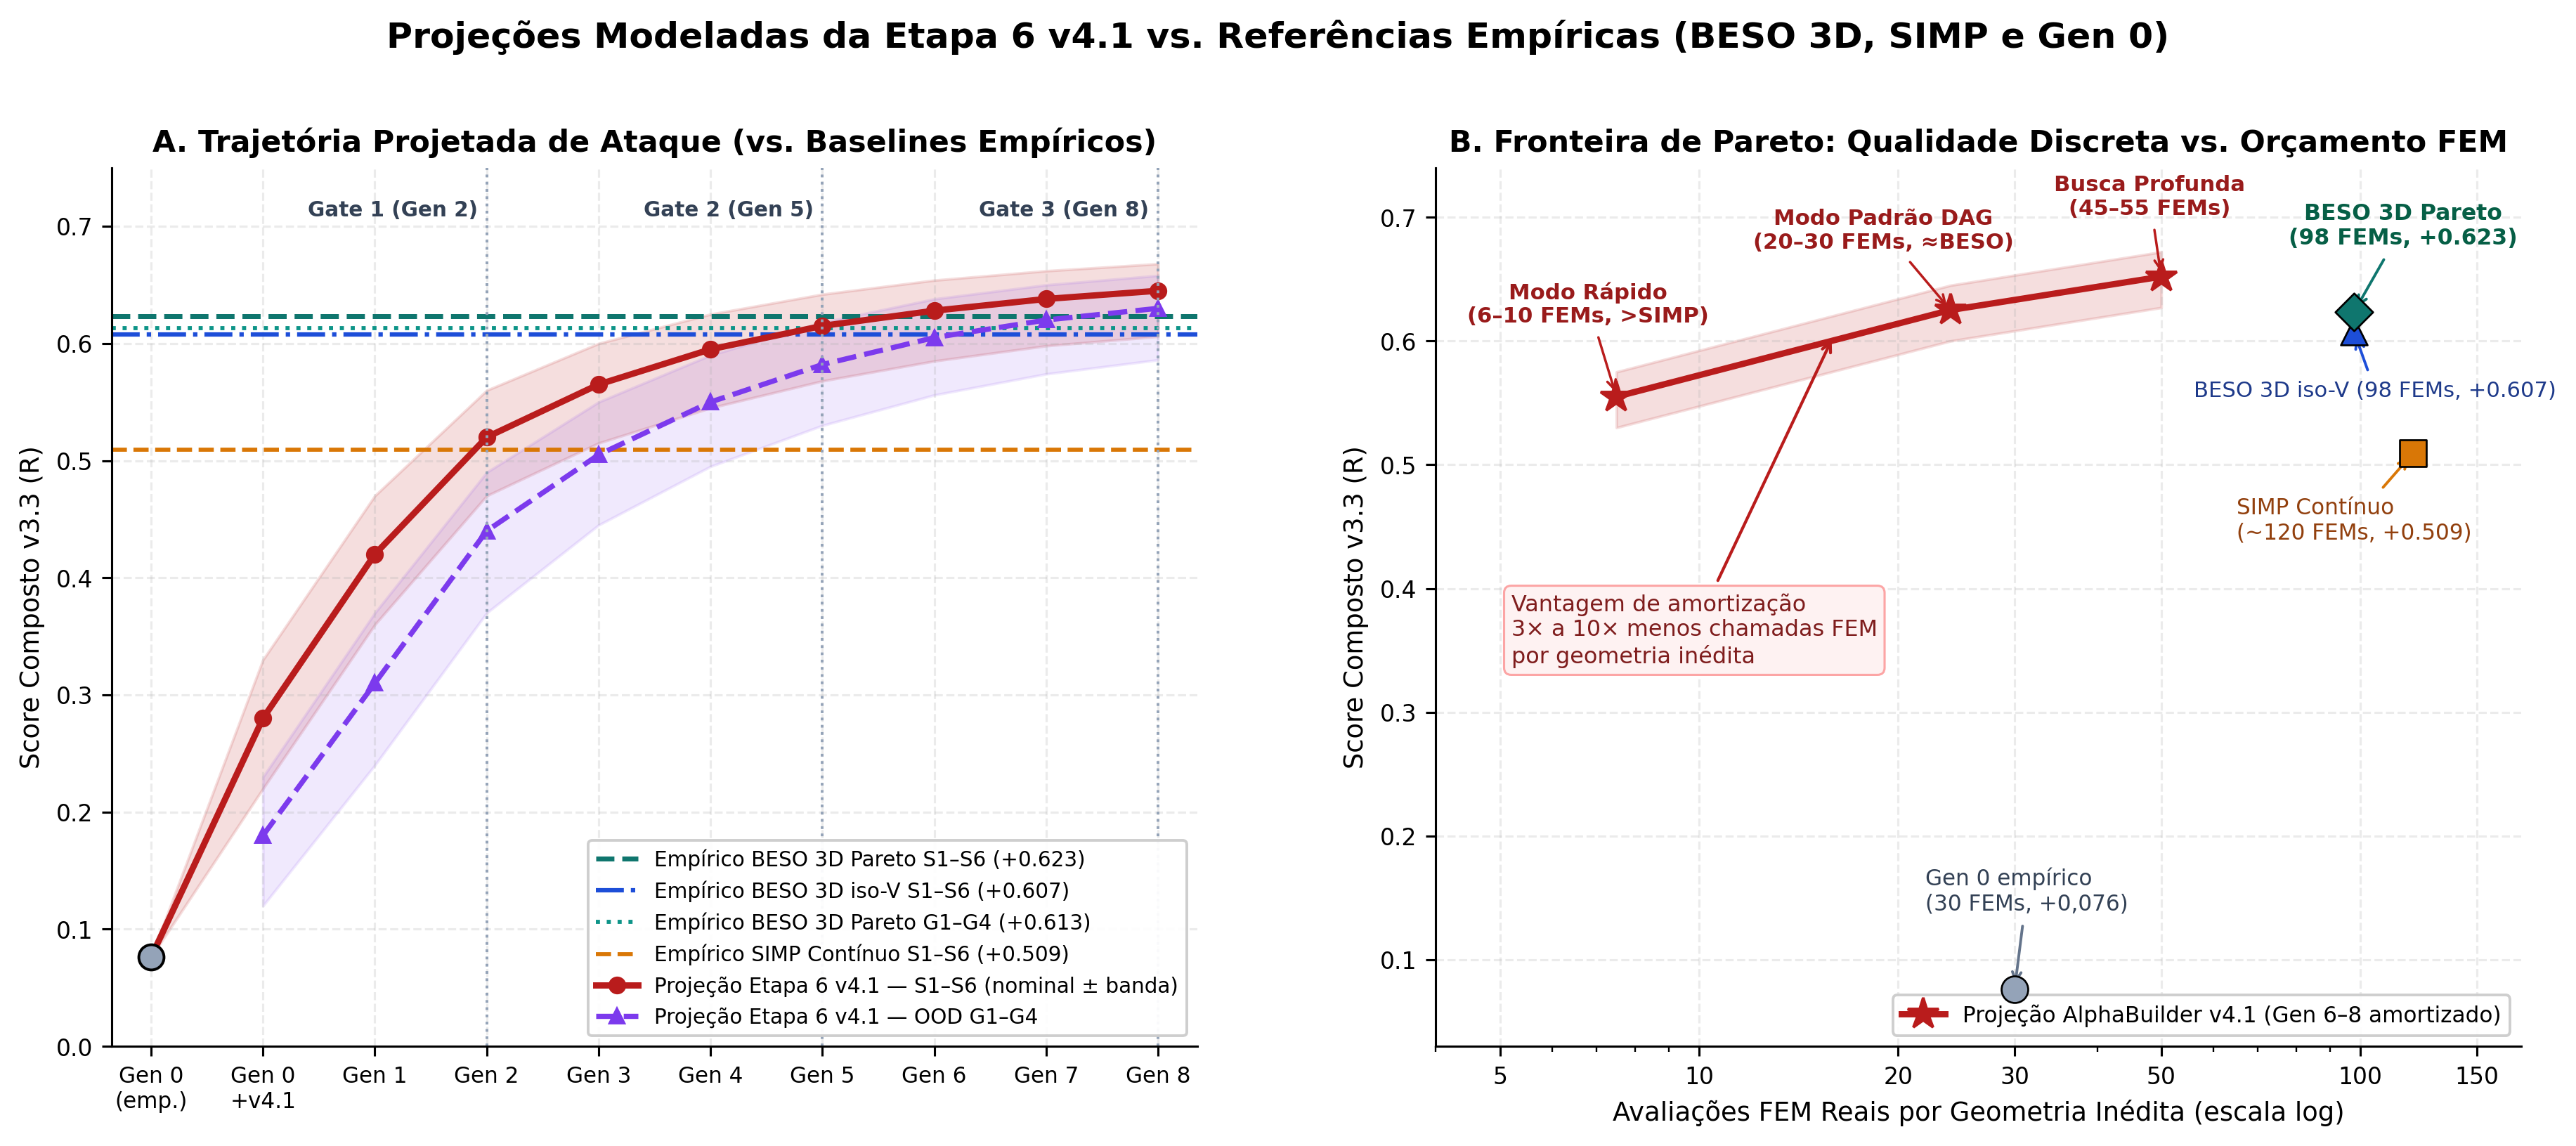
\includegraphics[width=0.98\linewidth]{fig_sota04_stage6_attack_projections.png}
  \caption{Projeções modeladas da trajetória da campanha Stage 6 \texttt{v4.1} sobre as referências empíricas medidas (Painel A) e posicionamento projetado na fronteira de Pareto entre Escore Composto \texttt{v3.3} e número real de avaliações FEM por nova geometria (Painel B).}
  \label{fig:sota04}
\end{figure}

\subsection{Portões de Decisão Falsificáveis (\textit{Go / Pivot Gates})}

Para manter o rigor experimental durante a execução das gerações em GPU, a Tabela~\ref{tab:gates} fixa critérios quantitativos explícitos e ações determinísticas caso qualquer etapa não atinja o desempenho esperado.

\begin{table}[htbp]
\centering
\caption{Portões de auditoria empírica e ações de pivô ao longo da campanha de auto-jogo da Etapa 6 \texttt{v4.1}.}
\label{tab:gates}
\resizebox{\textwidth}{!}{%
\begin{tabular}{@{}llll@{}}
\toprule
\textbf{Marco (Geração)} & \textbf{Critério Mínimo (\textit{Go})} & \textbf{Meta Nominal} & \textbf{Pivô Técnico Caso Falhe (\textit{No-Go})} \\
\midrule
\textbf{Gate 0} (Ablação \texttt{Gen 0+v4.1}) &
  \texttt{REM\%} P2 $> 15\%$ e \texttt{S1}--\texttt{S6} $> +0{,}20$ &
  $+0{,}25$ a $+0{,}33$ sem retreino &
  Elevar \texttt{remove\_prior\_floor} ($0{,}25 \to 0{,}35$) e peso \texttt{SWAP} \\
\textbf{Gate 1} (\texttt{Gen 2}, $\approx 128$ eps.) &
  Vencer \texttt{SIMP\_cont} ($+0{,}509$) em \texttt{S1}--\texttt{S6}; P1 $\ge 85\%$ &
  $+0{,}52$ (\texttt{S1}--\texttt{S6}); $+0{,}44$ (\texttt{G1}--\texttt{G4}) &
  Ampliar \textit{probes} contrafactuais \texttt{SED} no replay misto \\
\textbf{Gate 2} (\texttt{Gen 5}, $\approx 320$ eps.) &
  \texttt{S1}--\texttt{S6} $> +0{,}58$; \texttt{STOP\%} $> 25\%$; MAE $\log_{10}C < 0{,}35$ &
  $+0{,}615$ (alcance \texttt{BESO iso-V}) &
  Elevar \texttt{max\_phase2\_steps} ($64 \to 80$) e simulações P2 ($240$) \\
\textbf{Gate 3} (\texttt{Gen 8}, $\approx 512+$ eps.) &
  Bater \texttt{BESO Pareto} ($+0{,}623$ ou $+0{,}613$ OOD) em $\le 35$ FEMs &
  $+0{,}645$ \texttt{S1}--\texttt{S6}; vitória \texttt{G1}/\texttt{G3} ($3\text{--}5\times$ menos FEM) &
  Polimento híbrido: 1--2 passos BESO sobre saída da rede \cite{yi2026reinforcement} \\
\bottomrule
\end{tabular}%
}
\end{table}

Como linha de salvaguarda final prevista no \textbf{Gate 3}, caso a busca neural pura sature ligeiramente abaixo do teto de compliance fina em cantilevers clássicas ($< 0{,}02$ em escore), a arquitetura permanece compatível com um modo híbrido onde a rede neural fornece o campo $0/1$ inicial já oco em 10 a 20 chamadas e 1 a 2 passos finais de sensibilidade local executam o polimento de contorno — unificando a velocidade amortizada do Deep RL com a precisão local do gradiente exato.

\bibliographystyle{unsrtnat}
\bibliography{tcc/referencias}

\end{document}
